\chapter{Pengelolaan File CSV}

\section{Teori}
\section{Fungsi FIle CSV, Sejarah, dan Contoh}
File csv (comma separated value) sering digunakan dalam dunia pemrograman untuk menampilkan data. file csv memiliki format yang sangat sederhana, setiap baris dipisahkan oleh enter dan setiap kolom dipisahkan oleh tanda koma.\\
Kegunaan file csv dibandingkan file dengan format lainnya adalah dari segi kompatibilitas karena file csv dapat diolah, dimodifikasi, digunakan, import/export menggunakan berbagai software dan bahasa pemrograman, salah satunya pyhton.\\
Contoh file csv:\\
\lstinputlisting[caption=Contoh CSV, firstline=1, lastline=11]{src/FCSV.csv}
Contoh kode program python untuk membaca file csv.\\
\lstinputlisting[caption=Contoh Kode Python to Read CSV, language=python, firstline=1, lastline=6]{src/fcsv.py}
Contoh kode program python untuk membaca file csv menggunakan library pandas.\\
\lstinputlisting[caption=Contoh Kode Python to Read CSV, language=python, firstline=20, lastline=22]{src/fcsv.py}
Sejarah CSV.\\
CSV sudah digunakan sejak tahun 1972, CSV dapat dikompilasi pada bahasa pemrograman IBM Fortran. Data yang dipisahkan oleh koma apabila terdapat spasi didalamnya maka harus diberi tanda petik di awal dan akhir isi dari data tersebut. Nama CSV digunakan pada tahun 1983. Pada panduan dari Osborne Executive Computer terdapat kutipan yang membolehkan isi karakter memiliki koma. Pada tahun 2005 dengan RFC4180, CSV didefinisikan sebagai MIME Content Type. Lalu pada tahun 2013, defisiensi dari RFC4180 dipecahkan oleh rekomendasi dari W3C. Pada tahun 2014, IETF mempublikasi RFC7111 yang mendeskripsikan pecahan Uniform Resource Identifier(URI) ke dokumen CSV. RFC7111 menjelaskan tentang bagaimana baris, kolom dapat digunakan dalam dokumen CSV menggunakan indeks posisi. Pada Tahun 2015, W3C mempublikasikan draft rekomendasi untuk CSV-metadata standard yang dimulai pada bulan Desember 2015. 
\section{Aplikasi yang bisa Menciptakan File CSV}
Aplikasi yang dapat kita gunakan untuk membuat file csv ada banyak, diantaranya:
\begin{enumerate}
 \item Spreadsheet \linebreak Spreadsheet merupakan aplikasi pembuatan file CSV dengan cara memasukan data sesuai baris dan kolom yang diinginkan. Contoh spreadsheet seperti Google Spreadsheet, Microsoft Excel, dan aplikasi lainnya. 
 \item Bahasa Pemrograman \linebreak Bahasa pemrograman merupakan media untuk membuat aplikasi yang dapat digunakan untuk membuat file CSV khusus dengan bahasa pemrograman tertentu yang support dengan pembuatan file CSV. Seperti Python, C Sharp, dan lain sebagainya.
 \item Notepad atau Text Editor \linebreak Text editor juga dapat membuat file CSV, cukup dengan membuat file sesuai format CSV dan save file tersebut dengan ekstensi .csv.
\end{enumerate}

\section{Menulis dan Membaca File CSV pada Ms.Excel}
Membuat file csv melalui ms.excel sangatlah mudah, isikan nomor pada kolom, kemudian isikan variabel sebagai judul pada baris, lalu isikan data sesuai dengan variabel yang telah ditentukan, contoh:\\
\begin{figure}[H]
        \centerline{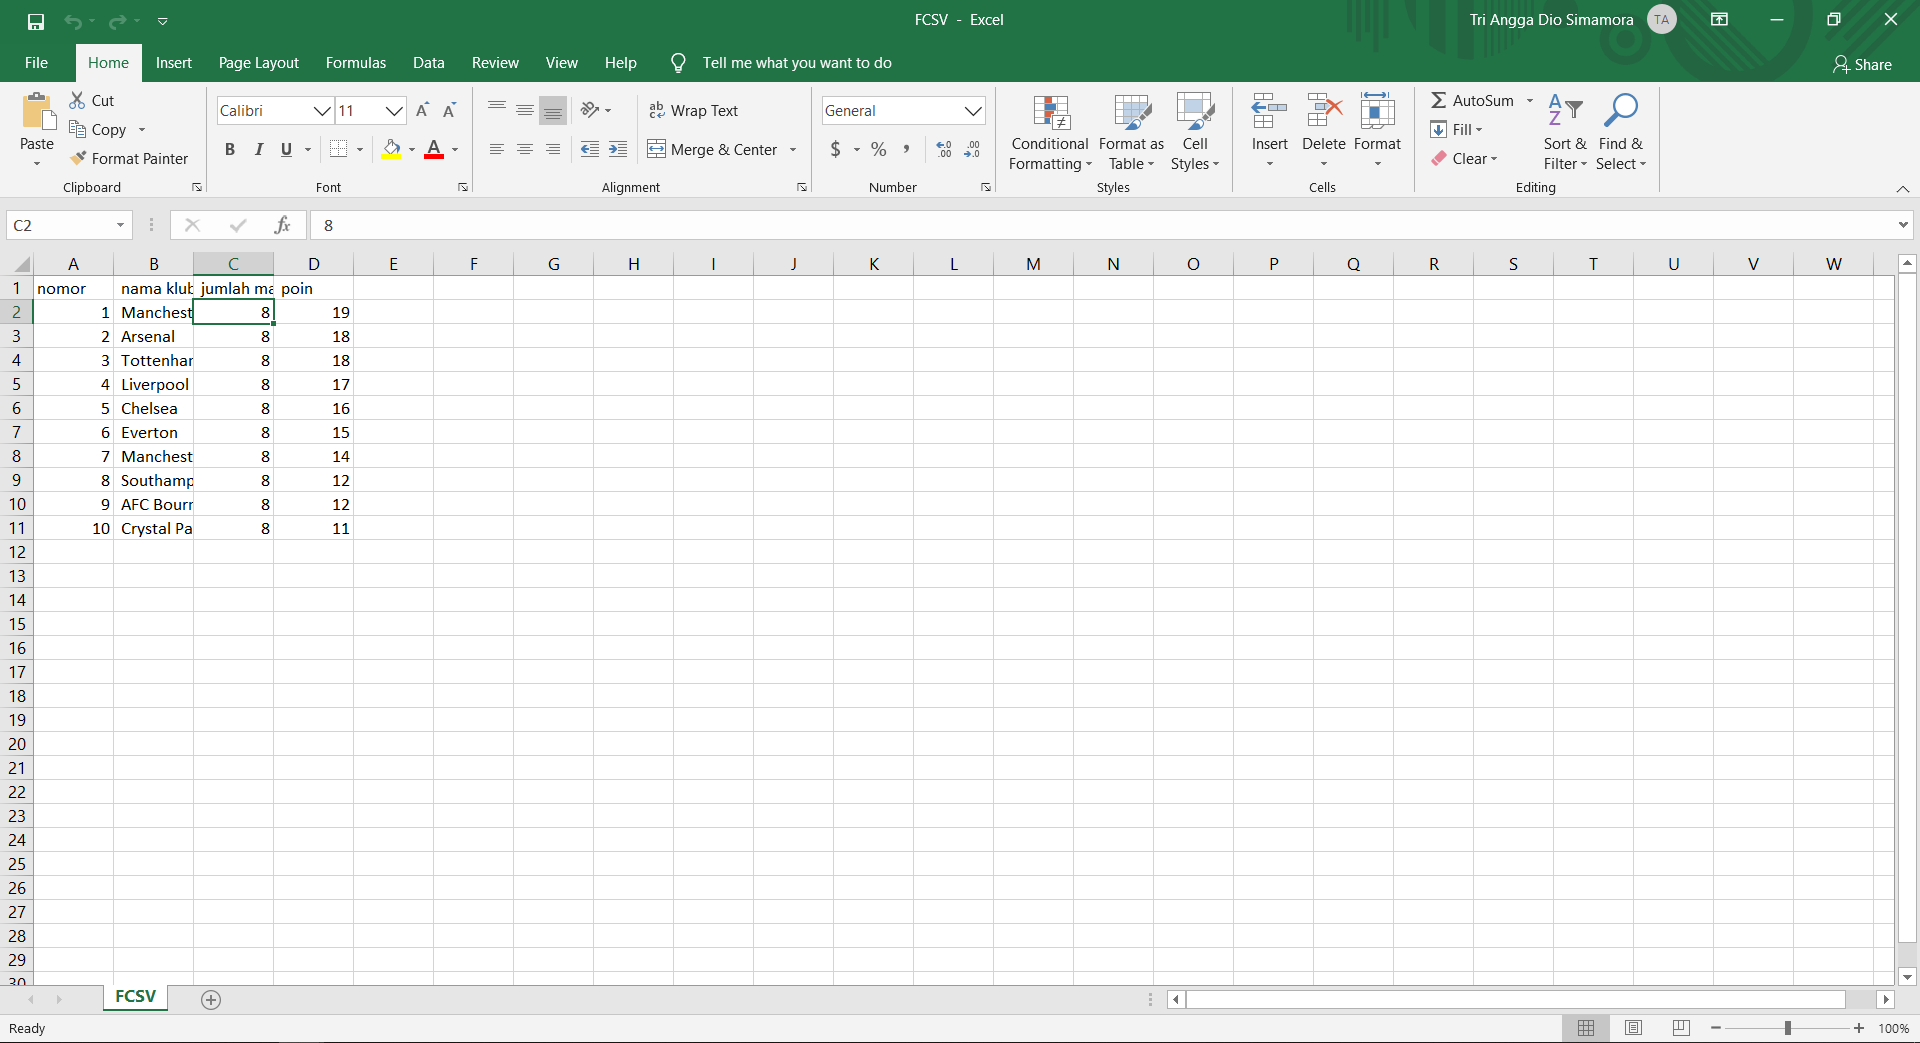
\includegraphics[scale=0.3]{figures/contoh}}
        \caption{Contoh Penulisan CSV pada Excel}
		\label{contoh}
\end{figure}
Setelah mengetikkan data pada excel, lalu pilih menu file, pilih menu export, pilih menu change file type, pilih csv, lalu klik tombol save as. Maka file excel akan menjadi file csv.
\lstinputlisting[caption=Contoh CSV, firstline=1, lastline=11]{src/FCSV.csv}


\subsection{Sejarah Library CSV}
Library CSV pada python merupakan library yang paling umum untuk import export data pada spreadsheet dan basis data dengan format sesuai dengan standarisasi RFC4180. Seiring dengan lahirnya bahasa pemrograman python, library mulai dibuat dan dikembangkan sampai akhirnya pada tahun 2003, Kevin Altis dan lainnya telah merilis versi final untuk library Python CSV. 

\subsection{Sejarah Library Pandas}
Pandas (Python Data Analysis Library) adalah library open source yang digunakan untuk melakukan data manajemen dan data analysis. Pandas diciptakan pada tahun 2008 oleh Wes McKinney dan diperbaharui oleh Sien Chang pada tahun 2010. Inspirasi dari pembuatan pandas muncul pada komunitas yang membutuhkan library khusus untuk analisis data.

\subsection{Fungsi - fungsi yang terdapat di library CSV}
Berikut fungsi-fungsi yang terdapat pada library csv.
\begin{enumerate}
\item \begin{verbatim} csv.reader(csvfile, dialect='excel', **fmtparams) \end{verbatim} Untuk mengembalikan	object reader yang akan mengambil setiap line pada csv. Data setiap baris diambil saat next() dipanggil. Berikut contohnya : \lstinputlisting[language=python, firstline=1, lastline=7]{src/fcsv.py}
 \item \begin{verbatim} csv.writer(csvfile, dialect='excel', **fmtparams) \end{verbatim} Mengembalikan file pembuat object untuk dapat mengkonversi data pada python ke file CSV yang akan dibuat. Berikut contoh penggunaan csv.writer : \lstinputlisting[language=python, firstline=9, lastline=18]{src/fcsv.py}
 \item \begin{verbatim} csv.register_dialect(name[, dialect[, **fmtparams]]) \end{verbatim} Mengasosiasikan dialek dengan nama, nama yang dimasukkan harus berupa karakter.
 \item \begin{verbatim} csv.unregister_dialect(name) \end{verbatim}
	Menghapus asosiasi dialek dengan nama pada registry dialek.
 \item \begin{verbatim} csv.get_dialect(name) \end{verbatim}
	Mengambil dialek yang telah diasosiasikan dengan nama. 
 \item \begin{verbatim}  csv.list_dialects() \end{verbatim} Mengembalikan dialek yang telah diregistrasi.
 \item \begin{verbatim} csv.field_size_limit([new_limit]) \end{verbatim} Mengembalikan maksimal kolom data yang diperbolehkan oleh pembaca.
\end{enumerate}

\subsubsection{Fungsi - fungsi yang terdapat di library Pandas}
\begin{enumerate}
 \item \begin{verbatim} pandas.read_csv(filepath_or_buffer[, sep, …]) \end{verbatim} Untuk membaca file CSV dan menyimpannya ke DataFrame. Contohnya: \lstinputlisting[language=Python, firstline=20, lastline=22]{src/fcsv.py}
 \item \begin{verbatim} pandas.read_excel(io[, sheet_name, header, names, …])  \end{verbatim} Membaca file excel dan menyimpannya ke DataFrame. Contohnya: \lstinputlisting[language=Python, firstline=24, lastline=26]{src/fcsv.py}
 \item \begin{verbatim} to_csv([path, index, sep, na_rep, …]) \end{verbatim}
	Untuk membuat file CSV dari data yang ada
\end{enumerate}

\section{Keterampilan Pemrograman}
\subsection{CSV List}
\lstinputlisting[caption=CSV List, language=Python, firstline=1, lastline=14]{src/D1184011_csv.py}
\subsection{CSV Dictionary}
\lstinputlisting[caption=CSV Dictionary, language=Python, firstline=16, lastline=27]{src/D1184011_csv.py}
\subsection{Hello NPM (Pandas List)}
\lstinputlisting[caption=Pandas List, language=Python, firstline=1, lastline=5]{src/D1184011_pandas.py}
\subsection{Hello NPM (Pandas Dictionary)}
\lstinputlisting[caption=Pandas Dictionary, language=Python, firstline=7, lastline=10]{src/D1184011_pandas.py}
\subsection{Pandas Date}
\lstinputlisting[caption=Pandas Date, language=Python, firstline=12, lastline=15]{src/D1184011_pandas.py}
\subsection{Pandas Ubah Index}
\lstinputlisting[caption=Pandas Ubah Index, language=Python, firstline=17, lastline=21]{src/D1184011_pandas.py}
\subsection{Pandas Ubah Column}
\lstinputlisting[caption=Pandas Ubah Column, language=Python, firstline=23, lastline=26]{src/D1184011_pandas.py}
\subsection{Main CSV}
\lstinputlisting[caption=Main CSV, language=Python, firstline=1, lastline=4]{src/main2.py}
\subsection{Main Pandas}
\lstinputlisting[caption=Digit Genap NPM, language=Python, firstline=1, lastline=7]{src/main3.py}
